\let\negmedspace\undefined
\let\negthickspace\undefined
\documentclass[journal]{IEEEtran}
\usepackage[a5paper, margin=10mm, onecolumn]{geometry}
%\usepackage{lmodern} % Ensure lmodern is loaded for pdflatex
\usepackage{tfrupee} % Include tfrupee package

\setlength{\headheight}{1cm} % Set the height of the header box
\setlength{\headsep}{0mm}     % Set the distance between the header box and the top of the text

\usepackage{gvv-book}
\usepackage{gvv}
\usepackage{cite}
\usepackage{amsmath,amssymb,amsfonts,amsthm}
\usepackage{algorithmic}
\usepackage{graphicx}
\usepackage{textcomp}
\usepackage{xcolor}
\usepackage{txfonts}
\usepackage{listings}
\usepackage{enumitem}
\usepackage{mathtools}
\usepackage{gensymb}
\usepackage{comment}
\usepackage[breaklinks=true]{hyperref}
\usepackage{tkz-euclide} 
\usepackage{listings}
% \usepackage{gvv}                                        
\def\inputGnumericTable{}                                 
\usepackage[latin1]{inputenc}                                
\usepackage{color}                                            
\usepackage{array}                                            
\usepackage{longtable}                                       
\usepackage{calc}                                             
\usepackage{multirow}                                         
\usepackage{hhline}                                           
\usepackage{ifthen}                                           
\usepackage{lscape}
\begin{document}
\bibliographystyle{IEEEtran}
\renewcommand{\thefigure}{\theenumi}
\renewcommand{\thetable}{\theenumi}
\setlength{\intextsep}{10pt} % Space between text and floats
\numberwithin{equation}{enumi}
\numberwithin{figure}{enumi}
\renewcommand{\thetable}{\theenumi}
\title{ASSIGNMENT-2}
\author{AI24BTECH11016-Jakkula Adishesh Balaji}
\maketitle
\bigskip
\section*{\textbf{Vector Arithmetic(Rank)}}
         \parindent 0px
         Question\brak{1.6.4} Show that the vectors $2\hat{i}-3\hat{j}+4\hat{k}$ and $-4\hat{i}+6\hat{j}-8\hat{k}$ are collinear.\\
\solution We have the vectors \\ \\
         \begin{table}[h!]
         	\centering
         	\begin{tabular}[12pt]{ |c| c|}
    \hline
    Parameter & Description\\ 
    \hline
    $P$ & $\myvec{2\\-3}$ \\
    \hline 
    $Q$ & $\myvec{10\\y}$ \\
    \hline
    $D$ & $Q-P$\\
    \hline 
    Distance & $10$ \\
    \hline
    \end{tabular}

         	\label{tab1.6.2.2}
         \end{table}
\\  
The matrix 
         \begin{align}
         {\myvec{A&B}}^{T} =
         \myvec{2&-3&4\\-4&6&-8} \\
         \xleftrightarrow{\text{$R_2=R_2+2R_1$}}
         \myvec{2&-3&4\\0&0&0}\\
         \end{align}
         which has rank 1. Hence, we conclude the given vectors are collinear
         \begin{figure}[h]
         	\centering
         	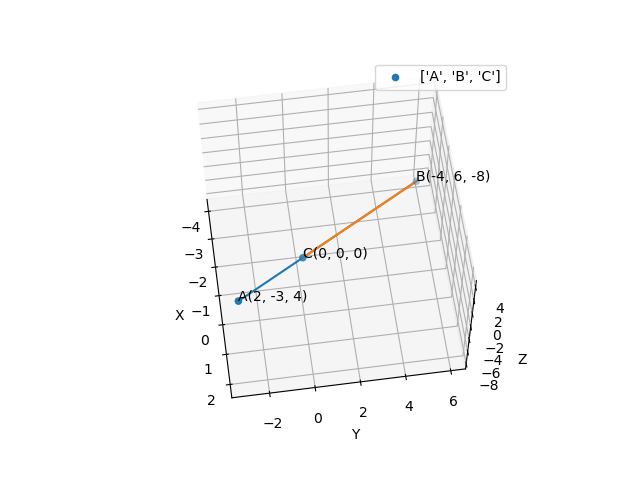
\includegraphics[width=\columnwidth]{figs/Figure.png}
         	\caption{Plot of $\vec{A}$,$\vec{B}$}
 	 \end{figure}
\end{document}                            
